\documentclass{if-beamer}
\usepackage{tikz-cd}
\usepackage[backend=bibtex,style=authoryear,sorting=none,maxcitenames=2, mincitenames=1, maxbibnames=4, uniquelist=false]{biblatex}
% \addbibresource{zotero_truncated.bib}
\addbibresource{QFT.bib}
% --------------------------------------------------- %
%                  Presentation info	              %
% --------------------------------------------------- %
\title[]{BCFW Recursion Relations}
\subtitle{Exchange Program at TU Dortmund, Summer 2025}
\author[Liu]{Xiaoyu Liu} % Add the second author here
\institute[Purdue]{Purdue University \and \textbf{Supervised by Prof. Emmanuel Stamou}}

\begin{document}

\begin{frame}
  \titlepage
\end{frame}

% --- Slide 1 --------------------------------------------------


\begin{frame}{TU Dortmund HET Group}
  \begin{figure}
    \centering
    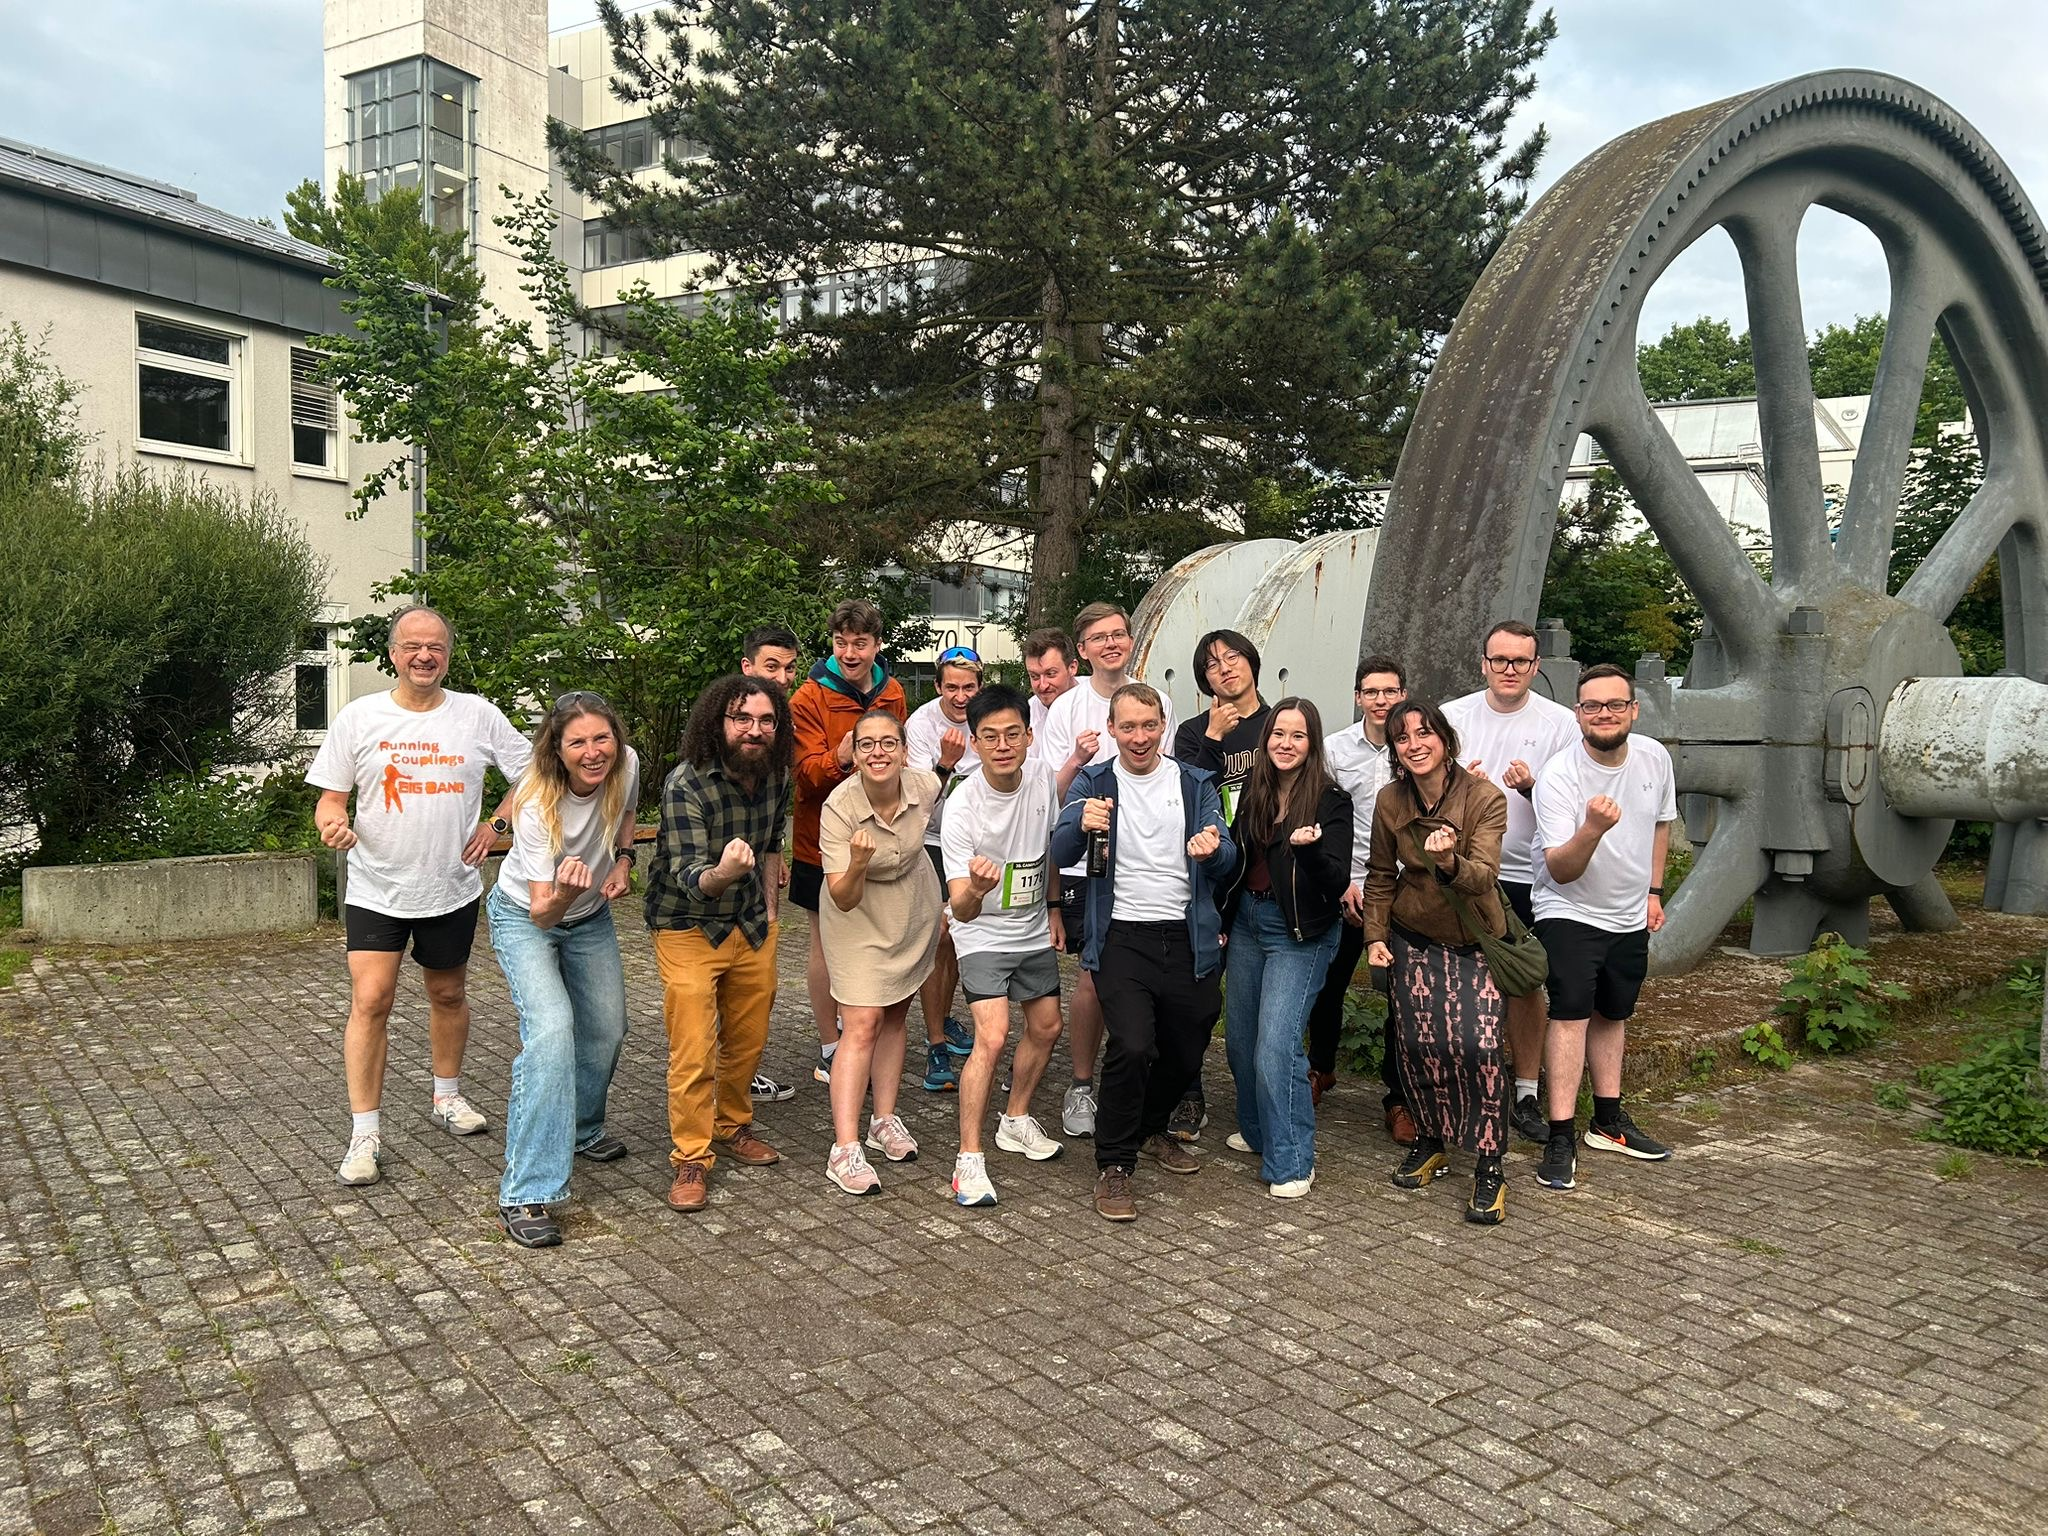
\includegraphics[width=0.6\linewidth]{src/marathon.JPG}
    \caption{A group photo of some members in the research team during campus Marathon.}
\end{figure}
\end{frame}


\begin{frame}{Background}
    \begin{itemize}
  \item \textbf{Explosion of Feynman diagrams}
    \begin{itemize}
      \item $gg\!\to\!gg$ (tree): $4$ diagrams; one--loop: $\sim220$ diagrams.
      \item $n$-gluon tree amplitudes: $n=6\!:\;220$ diagrams, $n=8:\;10\,480$.
    %   \item $pp\!\to\!3$ jets at NLO: $\mathcal{O}(10^4)$ diagrams.
    \end{itemize}
  \item \textbf{Yet the answers are simple}
    \begin{itemize}
      \item Parke--Taylor MHV amplitude (all $+$ except two $-$ helicities): one-line formula valid for any~$n$.
    \[
    \mathcal{A}\left(1^{+} \cdots i^{-} \cdots j^{-} \cdots n^{+}\right)=i(-g)^{n-2} \frac{\langle i j\rangle^4}{\langle 12\rangle\langle 23\rangle \cdots\langle(n-1) n\rangle\langle n 1\rangle}
    \]
      \item Simplicity hints at hidden symmetries and geometric structures invisible to brute‑force perturbation.
    \end{itemize}
  \item \textbf{Why pursue on‑shell methods?}
    \begin{itemize}
      \item \emph{Theoretical}: getting us closer to non-perturbative QFT.
      \item \emph{Computational}: orders‑of‑magnitude speed‑up for both symbolic and numerical evaluation of amplitudes.
      (Caveats)
    \end{itemize}
\end{itemize}
\end{frame}

% --- Slide 2 --------------------------------------------------
\begin{frame}{Polology and Factorization}
\begin{itemize}
  \item Momentum–space $n$‑point Green’s function: $G_n(p_1,\dots,p_n)$.
  \item \textbf{Polology theorem}\,: If $p^2=(p_1\!+\!\dots+\!p_r)^2=m^2$ and the one‑particle matrix element \mbox{$\langle\Psi|\phi\dots\phi|\Omega\rangle\neq0$}, then $G_n$ has a simple pole at~$p^2=m^2$ and factorizes.
  \[
\begin{aligned}
G = & \frac{-2 i \sqrt{\mathbf{p}^2+m^2}}{p^2+m^2-i \epsilon}(2 \pi)^7 \delta^4\left(p_1+\cdots+p_n\right) \\
& \times \sum_\sigma M_{0 \mid \mathbf{p}, \sigma}\left(p_2 \cdots p_r\right) M_{\mathbf{p}, \sigma \mid 0}\left(p_{r+2} \cdots p_n\right)\\
& + \text { terms regular at } p^2=m^2.
\end{aligned}
\]
\end{itemize}
\begin{figure}
    \centering
    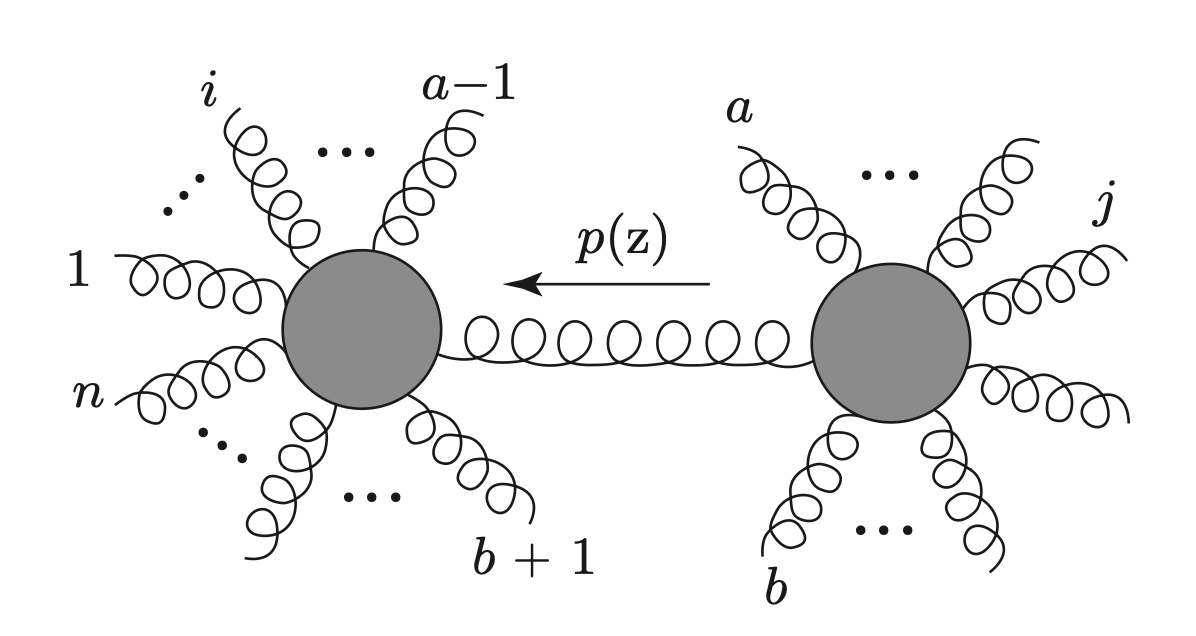
\includegraphics[width=0.5\linewidth]{src/Schwartz27-2.png}
    \caption{Schwartz (2014) Figure 27.2: Factorization Channel}
\end{figure}
\end{frame}

% --- Slide 3 --------------------------------------------------
\begin{frame}{Spin–Helicity \& Three‑Point Amplitudes}
\begin{itemize}
    \item Spinors: $|p\rangle$ for left-handed, $[p|$ for right-handed. They are from the $(\frac{1}{2}, \frac{1}{2})$ representation of the Lorentz group.
  \item Massless $p^\mu$ written as bispinor $p^{\alpha\dot\alpha}=|p\rangle[p|$ with $p^2=0$.
  \item Little‑group scaling invariance: $|p\rangle\!\to z|p\rangle$, $[p|\to z^{-1}[p|$.
  \item Gluon polarizations: $\epsilon^-\!\sim|p\rangle[r|/[pr]$ scales $z^2$, $\epsilon^+\!\sim|r\rangle[p|/\langle rp\rangle$ scales $z^{-2}$.
  \item Dimensional \& scaling analysis $\Rightarrow$ unique (up to colour factor $C^{abc}$) 3‑pt forms:
  \begin{align*}
    \mathcal{M}(1^{+}2^{+}3^{+})&=C^{abc}[12][23][31], \qquad
    \mathcal{M}(1^{+}2^{+}3^{-})=C^{abc}\frac{[12]^3}{[13][32]},\qquad\\
    \mathcal{M}(1^{-}2^{-}3^{+})&=C^{abc}\frac{\langle12\rangle^{3}}{\langle13\rangle\langle32\rangle}.
  \end{align*}
\end{itemize}
\end{frame}


% --- Slide 4 --------------------------------------------------
\begin{frame}{BCFW Shift and Recursion Formula (2005)}
\cite{Britto:2005fq}
\begin{itemize}
  \item Choose legs $i<j$ and complexify the momenta via a BCFW shift: 
  \[
     |\hat{j}\rangle=|j\rangle-z|i\rangle,\quad[\hat{i}|=[i|+z[j|,\quad z\in\mathbb{C}.
  \]
  \item $\hat p_i,\hat p_j$ remain massless and momentum is conserved $\Rightarrow\mathcal{M}(z)$ analytic with simple poles.
  \item Each pole $z=z_{a,b}^*$ where an internal momentum \mbox{$\hat P(z)^2\!=\!0$} gives local factorization
  \[
     -\frac1{z^*}\operatorname{Res}_{z=z^*}\mathcal{M}(z)=\mathcal{M}_L(z^*)\,\frac{1}{P^2}\,\mathcal{M}_R(z^*).
  \]
  \item Contour $\oint\!dz\,\mathcal{M}(z)/z$ (with $\mathcal{M}(z)\to0$ as $|z|\to\infty$) yields the on‑shell BCFW recursion\;
  \[
  \mathcal{M}(1\dots n)=\sum_{a,b,h}\mathcal{M}_L(\hat P^h)\,\frac{1}{P_{a\dots b}^2}\,\mathcal{M}_R(\hat P^{-h}).
  \]
\end{itemize}
\end{frame}


% --- Slide 4.5 --------------------------------------------------

\begin{frame}{Gauge Invariance and Examples}
\begin{itemize}
  \item Gauge invariance: the choice of reference vectors $|r\rangle$ and $[r|$, in the polarizations
  \[
    \epsilon^-(p,r)=\frac{|p\rangle[r|}{\langle pr\rangle},\quad
    \epsilon^+(p,r)=\frac{|r\rangle[p|}{\langle rp\rangle},
  \]
  does not affect the physical amplitude.
  \item In particular, the choice of $\epsilon_1 = \epsilon(p_1, p_2)$ and $\epsilon_2 = \epsilon(p_2, p_1)$ makes $p_1 + p_2$ channel vanish, since $\epsilon_1 \cdot \epsilon_2 = \epsilon_1 \cdot p_2 = \epsilon_2 \cdot p_1 = 0$.
  \item In BCFW, we choose $r_i = p_j$ and $r_j = p_i$.
\end{itemize}
\begin{example}
  Consider $g_1g_2 \to g_3g_4$ in color-ordered QCD. At tree-level perturbation theory we have $s$ and $t$ diagrams.

  Choose legs $i=1$ and $j=3$ and we have  ``killed'' the $t$-channel, leaving only the $s$-channel diagram (an onshell diagram, however.) Thus,
  \[
\widetilde{\mathcal{M}}\left(1^{-} 2^{-} 3^{+} 4^{+}\right)=-\frac{\langle\hat{1} 2\rangle^3}{\langle\hat{1} \hat{P}\rangle\langle\hat{P} 2\rangle} \frac{1}{\langle 12\rangle[21]} \frac{[3 \hat{4}]^3}{[3 \hat{P}][\hat{P} \hat{4}]} = 
\frac{\langle 12\rangle^4}{\langle 12\rangle\langle 23\rangle\langle 34\rangle\langle 41\rangle}.
\]
\end{example}

\end{frame}

% --- Slide 5 --------------------------------------------------
\begin{frame}{Planar View \& Generalizations}
\begin{block}{Planar Trees}
 In a planar theory with crossing symmetry (e.g. colour‑ordered QCD, $N \to \infty$ SYM) every tree diagram is planar. BCFW recursively enumerates connected planar trees, each contributing $g^{n-2}$ to the $n$‑point amplitude.
  \[
  \mathcal{M}(1\dots n)=\sum_{a,b,h}\mathcal{M}_L(\hat P^h)\,\frac{1}{P_{a\dots b}^2}\,\mathcal{M}_R(\hat P^{-h}).
  \]
\end{block}
\begin{block}{Extensions}
\begin{itemize}
  \item \textbf{Massive\,/\,higher‑spin:} Spin‑helicity extended to arbitrary spins\,\autocite{Arkani-Hamed:2017jhn}.
  \item \textbf{Off‑shell external legs:} All‑line and one‑line shifts\,\autocite{vanHameren:2014iua,Cohen:2024xuf}.
  \item \textbf{Loop level:} Planar $\mathcal{N}=4$ SYM recursion\,\autocite{Arkani-Hamed:2010zjl}; connection to amplituhedron.
\end{itemize}
\end{block}
% \begin{center}\small Further reading: Weinberg~(1995), Schwartz~(2014), Britto–Cachazo–Feng–Witten~(2005)\end{center}
\end{frame}

\begin{frame}{BCFW for QED}
  \begin{block}{The QED Amplitude}
    QED has no boson-only vertices, and all amplitudes have at least one fermion pair. 
  \end{block}
  \begin{block}{Symmetrization Relation}
  $$
  A^{\mathrm{QED}}(\bar{f}, f, 1,2,3, \ldots, n)=A(\bar{f}, f, 1,2,3, \ldots, n)+A(\bar{f}, f, 2,1,3, \ldots, n)+\cdots
  $$  
  [Ozeren and Stirling 2005] obtains MHV QED amplitude from symmetrization of color-ordered MHV QCD amplitude.  
  \end{block}
  \begin{itemize}
    \item This tells us that $SU(N)$ Yang-Mills is very simple at $N = 1$ and $N = \infty$ , and those two are related.
    \item The formula also tells us that QED, trivially, has recursion relations. The computational advantage may wane due to the sum over permutations involved. The BCFW in QCD only works in large-N limit where we have planarity; this is not true for QED, where tree-level amplitudes can be obtained via the symmetrization though we don't have planarity. Correspondingly, BCFW for QED has slightly different recursion rules and additional symmetrization terms.
  \end{itemize}

\end{frame}

\begin{frame}{Ccombinatorial structure of amplitudes (A glimpse)}
\begin{center}
  \begin{tabular}{cc}
    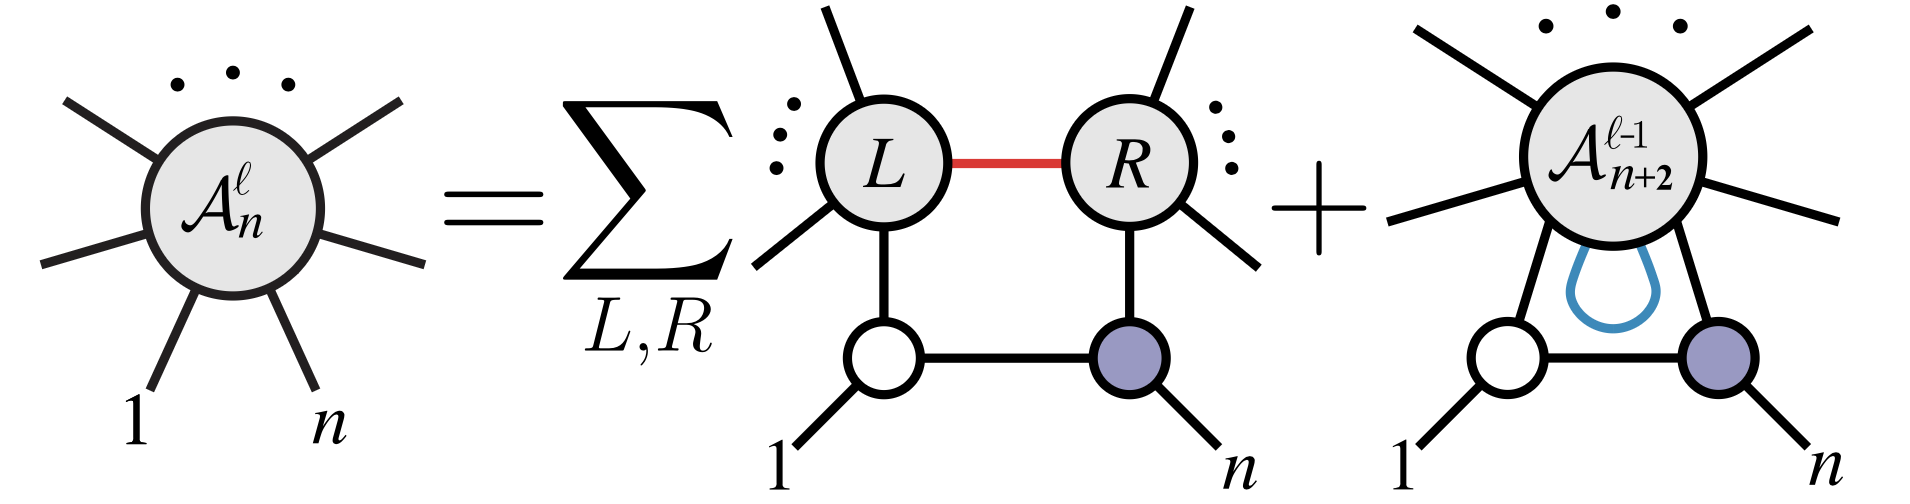
\includegraphics[width=0.5\linewidth]{src/Arkani-HamedGrassmannian2-25.png} &
    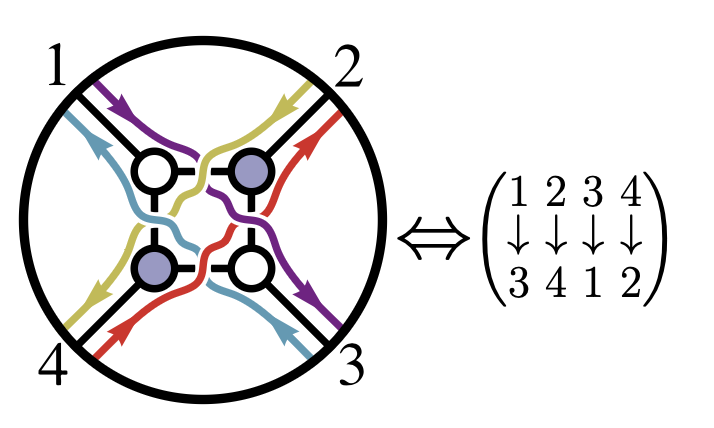
\includegraphics[width=0.3\linewidth]{src/Arkani-HamedGrassmannian3-5.png} \\
    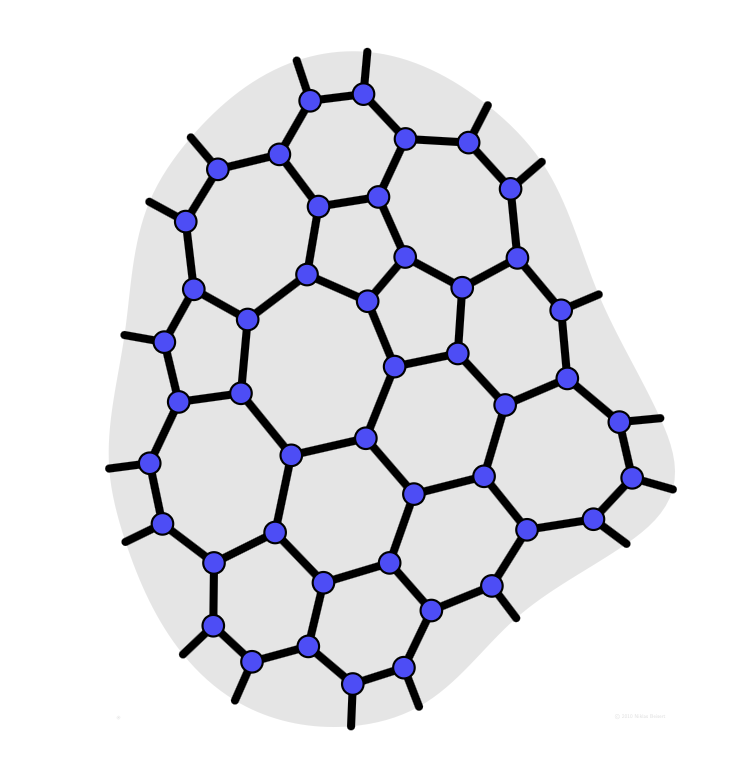
\includegraphics[width=0.3\linewidth]{src/Beisert-2012-2.png} &
    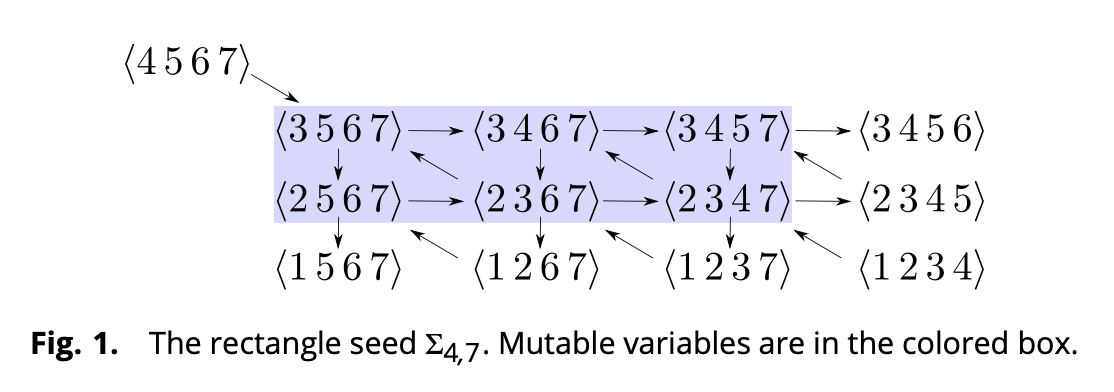
\includegraphics[width=0.45\linewidth]{src/EvenZohar1.png} \\
  \end{tabular}
\end{center}
\end{frame}

% \begin{frame}{Future Work}
% \begin{itemize}
%   \item BCFW for QED. The QED story should be similar to QCD, but with no gluon 3- and 4-vertex, but quark-gluon vertices. All machinery depends on the following formula for MHV amplitudes:
%   \[A^{\mathrm{QED}}\left(\bar{f}^{+}, f^{-}, 1^{+}, 2^{+} \ldots, I^{-}, \ldots, n^{+}\right)=\frac{2^{\frac{n}{2}} e^n\langle f \bar{f}\rangle^{n-2}\langle f I\rangle^3\langle\bar{f} I\rangle}{\prod_{k=1}^n\langle f k\rangle\langle\bar{f} k\rangle}.\]
%   \item Loop-level recursion. 
%   \item Massive BCFW.
%   \item Implementation of recursive algorithms for amplitudes.
% \end{itemize}

% \end{frame}

\begin{frame}{References}
\printbibliography[heading=none]
\end{frame}

\end{document}
